\documentclass[11pt,letterpaper]{article}

\usepackage[margin=1in]{geometry}
\usepackage{enumitem}
\usepackage{hyperref}
\usepackage{amsmath}
\usepackage{amssymb}
\usepackage{booktabs}
\usepackage{float}
\usepackage{tikz}
\usetikzlibrary{decorations.pathmorphing, decorations.pathreplacing, calc, arrows.meta}

\title{16.07 Dynamics Problem Set 5}
\author{Due Wednesday, November 11}
\date{}

% vector / matrix shorthands
\newcommand{\bw}{\boldsymbol{\omega}}
\newcommand{\bwd}{\boldsymbol{\omega}_d}
\newcommand{\bh}{\mathbf{h}}
\newcommand{\Bw}{{}^{B}\boldsymbol{\omega}}
\newcommand{\Bwd}{{}^{B}\boldsymbol{\omega}_d}
\newcommand{\Nht}{{}^{N}\mathbf{h}_{\text{tot}}}
\newcommand{\bJ}{\mathbf{J}}
\newcommand{\bQ}{\mathbf{Q}}
\newcommand{\bq}{\mathbf{q}}
\newcommand{\bx}{\mathbf{x}}

\begin{document}

\maketitle

\section*{Part 1: Error Analysis of the Bifilar Pendulum Lab}

\begin{figure}[h]
\centering
% ---------------- Left panel: oblique view of the suspended T-shaped body ----------------
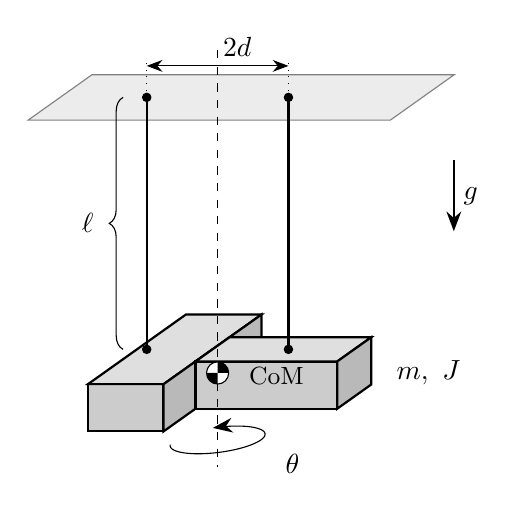
\begin{tikzpicture}[scale=1.0,
    x={(1cm,0cm)}, y={(0.45cm,0.32cm)}, z={(0cm,1cm)}]
    % 3D coordinates (x,y,z); z is up, x along the stem, origin directly above the body's CoM.
    % Drawing scale: 1 unit = 1/12 m, so d = 7.5 cm -> 0.9 units.
    \def\hd{0.9}    % d, half of the string separation
    \def\Ls{3.2}    % string length \ell (not to scale)
    \def\bh{0.6}    % body thickness (5 cm)
    \def\zt{-\Ls}           % top surface of the body
    \def\zb{-\Ls-\bh}       % bottom surface of the body

    % Ceiling
    \filldraw[fill=gray!15, draw=gray] (-2.0,-0.9,0) -- (2.6,-0.9,0) -- (2.6,0.9,0) -- (-2.0,0.9,0) -- cycle;

    % Box A (crossbar): x in [-1.0247,-0.0647], y in [-1.38,1.38]
    \filldraw[fill=gray!40, draw=black, thick]
        (-1.0247,-1.38,\zt) -- (-0.0647,-1.38,\zt) -- (-0.0647,-1.38,{\zb}) -- (-1.0247,-1.38,{\zb}) -- cycle;
    \filldraw[fill=gray!25, draw=black, thick]
        (-1.0247,-1.38,\zt) -- (-0.0647,-1.38,\zt) -- (-0.0647,1.38,\zt) -- (-1.0247,1.38,\zt) -- cycle;
    \filldraw[fill=gray!55, draw=black, thick]
        (-0.0647,-1.38,\zt) -- (-0.0647,1.38,\zt) -- (-0.0647,1.38,{\zb}) -- (-0.0647,-1.38,{\zb}) -- cycle;

    % Box B (stem): x in [-0.0647,1.7353], y in [-0.48,0.48]
    \filldraw[fill=gray!40, draw=black, thick]
        (-0.0647,-0.48,\zt) -- (1.7353,-0.48,\zt) -- (1.7353,-0.48,{\zb}) -- (-0.0647,-0.48,{\zb}) -- cycle;
    \filldraw[fill=gray!25, draw=black, thick]
        (-0.0647,-0.48,\zt) -- (1.7353,-0.48,\zt) -- (1.7353,0.48,\zt) -- (-0.0647,0.48,\zt) -- cycle;
    \filldraw[fill=gray!55, draw=black, thick]
        (1.7353,-0.48,\zt) -- (1.7353,0.48,\zt) -- (1.7353,0.48,{\zb}) -- (1.7353,-0.48,{\zb}) -- cycle;

    % Vertical axis through the CoM
    \draw[dashed] (0,0,0.6) -- (0,0,{\zb-0.9});

    % Strings
    \draw[thick] (-\hd,0,0) -- (-\hd,0,\zt);
    \draw[thick] (\hd,0,0) -- (\hd,0,\zt);
    \filldraw (-\hd,0,0) circle (1.5pt);
    \filldraw (\hd,0,0) circle (1.5pt);
    \filldraw (-\hd,0,\zt) circle (1.5pt);
    \filldraw (\hd,0,\zt) circle (1.5pt);

    % CoM marker (directly below the midpoint between the strings)
    \coordinate (CM) at (0,0,{-\Ls-\bh/2});
    \filldraw[fill=white] (CM) circle (4pt);
    \fill (CM) -- ++(4pt,0) arc (0:90:4pt) -- cycle;
    \fill (CM) -- ++(-4pt,0) arc (180:270:4pt) -- cycle;
    \node[font=\small, right] at ($(CM)+(0.32,-0.1)$) {CoM};

    % Separation 2d (dimension line above the ceiling)
    \draw[dotted] (-\hd,0,0) -- (-\hd,0,0.5);
    \draw[dotted] (\hd,0,0) -- (\hd,0,0.5);
    \draw[{Stealth[length=2mm]}-{Stealth[length=2mm]}] (-\hd,0,0.4) -- (\hd,0,0.4);
    \node[above] at (0.25,0,0.4) {$2d$};

    % String length \ell (brace to the left of the left string)
    \draw[decorate, decoration={brace, amplitude=5pt}]
        (-\hd-0.3,0,\zt) -- (-\hd-0.3,0,0);
    \node at (-\hd-0.75,0,{-\Ls/2}) {$\ell$};

    % Mass and inertia label
    \node[right] at (2.15,0,{-\Ls-\bh/2}) {$m,\ J$};

    % Twist angle about the vertical axis
    \draw[-{Stealth[length=2.5mm]}] plot[domain=200:480, samples=80, variable=\t]
        ({0.55*cos(\t)},{0.55*sin(\t)},{\zb-0.55});
    \node at (0.95,0,{\zb-0.85}) {$\theta$};

    % Gravity
    \draw[-{Stealth[length=2.5mm]}, thick] (3.0,0,-0.8) -- (3.0,0,-1.7);
    \node[right] at (3.0,0,-1.25) {$g$};
\end{tikzpicture}
\hspace{0.3cm}
% ---------------- Right panel: top view with the body twisted ----------------
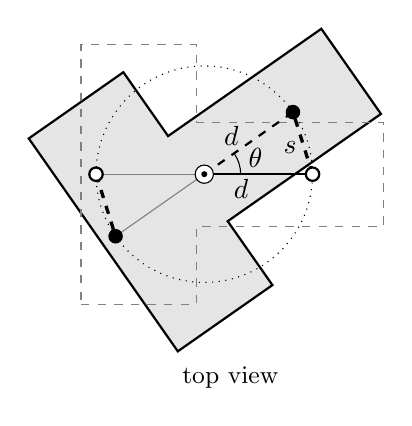
\begin{tikzpicture}[scale=1.1]
    % Drawing scale: d = 7.5 cm -> 1.25 units; the T outline is compressed to fit (not to scale). Origin at the body's CoM.
    \def\hd{1.25}   % d
    \def\th{35}     % twist angle shown
    \def\tshape{(-1.4232,-1.5) -- (-0.0899,-1.5) -- (-0.0899,-0.6) -- (2.07,-0.6) -- (2.07,0.6) -- (-0.0899,0.6) -- (-0.0899,1.5) -- (-1.4232,1.5) -- cycle} % T outline, compressed (not to scale)

    % Twisted body
    \begin{scope}[rotate=\th]
        \filldraw[fill=gray!20, draw=black, thick] \tshape;
    \end{scope}

    % Body outline at equilibrium
    \draw[dashed, gray] \tshape;

    % Circle of radius d traced by the body's string attachment points
    \draw[dotted] (0,0) circle (\hd);

    % Radii of length d: at rest (to the ceiling attachment) and twisted (to the body attachment)
    \draw[thick] (0,0) -- (\hd,0);
    \draw[thick, dashed] (0,0) -- ({\hd*cos(\th)},{\hd*sin(\th)});
    \draw[gray] (0,0) -- (-\hd,0);
    \draw[gray] (0,0) -- ({-\hd*cos(\th)},{-\hd*sin(\th)});

    % Horizontal projections of the strings (length s)
    \draw[very thick, dashed] (\hd,0) -- ({\hd*cos(\th)},{\hd*sin(\th)});
    \draw[very thick, dashed] (-\hd,0) -- ({-\hd*cos(\th)},{-\hd*sin(\th)});

    % Attachment points: open = ceiling (fixed), filled = body
    \filldraw[fill=white, thick] (\hd,0) circle (2.2pt);
    \filldraw[fill=white, thick] (-\hd,0) circle (2.2pt);
    \filldraw ({\hd*cos(\th)},{\hd*sin(\th)}) circle (2.2pt);
    \filldraw ({-\hd*cos(\th)},{-\hd*sin(\th)}) circle (2.2pt);

    % Labels for the d--d--s triangle
    \node[below, inner sep=1pt] at ({\hd/2-0.2},-0.02) {$d$};
    \node at ({0.55*\hd*cos(\th)-0.25},{0.55*\hd*sin(\th)+0.05}) {$d$};
    \node[inner sep=1.5pt] at ({\hd*cos(\th/2)-0.2},{\hd*sin(\th/2)-0.07}) {$s$};

    % Twist angle
    \draw (0.42,0) arc (0:\th:0.42);
    \node at ({0.62*cos(\th/2)},{0.62*sin(\th/2)}) {$\theta$};

    % Vertical axis (out of the page) through the CoM
    \filldraw[fill=white] (0,0) circle (3pt);
    \fill (0,0) circle (1pt);

    \node[font=\small] at (0.3,-2.35) {top view};
\end{tikzpicture}
\caption{The bifilar pendulum setup from Problem Set 3. Left: oblique view at rest; the strings attach to the top of the body on its $x$ axis, a distance $d$ on either side of the CoM. Right: top view with the body twisted by $\theta$ about the vertical axis through its center of mass (pointing out of the page). Open circles mark where the strings attach to the ceiling (fixed); filled circles mark where they attach to the body. The thick dashed segments of length $s$ are the horizontal projections of the strings. Drawings are not to scale.}
\label{fig:bifilar}
\end{figure}

\noindent In lab, you hung your 3D-printed T-shaped body as a bifilar pendulum (Fig.~\ref{fig:bifilar}) and timed its small twisting oscillations. In Problem Set 3, you showed that the yaw moment of inertia about the vertical axis through the center of mass is
\[
J = \frac{mgd^2P^2}{4\pi^2\ell},
\]
where $m$ is the mass of the body, $\ell$ is the string length, $2d$ is the string separation, and $P$ is the period of small oscillations. In this part, you'll use the data from your lab worksheet to compute $J$, estimate how uncertain that measurement is, and compare it with a prediction from the object's geometry.

Use your own recorded values of $m$, $\ell$, and $2d$, and your three timing trials, each measuring the time $t$ for 10 complete cycles. Work in CGS units, with $g = 981$~cm/s$^2$. Throughout, denote the uncertainty in a quantity $x$ by $\sigma_x$, and assume:
\begin{itemize}
    \item You measured the string length $\ell$ and the separation $2d$ with the measuring tape to within about $\pm 0.1$~cm. So $\sigma_\ell = 0.1$~cm, and since $d$ is half the measured separation, $\sigma_d = 0.05$~cm.
    \item Your phone stopwatch gives an uncertainty of about $\pm 0.1$~s on each timed interval, because of your reaction time, regardless of how long the interval is.
    \item The mass $m$ and $g$ are known precisely enough that their errors are negligible.
\end{itemize}

\subsection*{Measured Inertia and Its Uncertainty}

\begin{enumerate}[label=(\alph*)]
    \item \textbf{Measured inertia:} Report your measured values of $m$, $\ell$, $d$, and the three times $t$. Compute the period $P = t/10$ for each trial and the average period $\bar{P}$. Then use $\bar{P}$ to compute your measured moment of inertia $J$.

    \item \textbf{Error propagation:} For small errors, we can calculate the expected error in the output of a function by mapping the expected errors in the inputs through the function's derivative. If the error sources are independent, then we can combine them by adding them in quadrature (i.e., taking the root-sum-square, or RSS). For a function $z = f(x,y)$, we would have
    \[
    \sigma_z = \sqrt{\left( \frac{\partial f}{\partial x} \sigma_x \right)^2+ \left( \frac{\partial f}{\partial y} \sigma_y \right)^2}.
    \]
    Using the expression for $J$ above, derive an expression for the uncertainty $\sigma_J$ in terms of the uncertainties $\sigma_d$, $\sigma_\ell$, and $\sigma_P$. Then divide by $J$ to write the fractional uncertainty $\sigma_J/J$ in terms of $\sigma_d/d$, $\sigma_\ell/\ell$, and $\sigma_P/P$. Why do some measurements affect $\sigma_J/J$ more strongly than others, even when their fractional uncertainties are the same?

    \item \textbf{Timing a single period:} Suppose you had timed only a single oscillation, with the same stopwatch uncertainty. Using your values from part (a), compute the contribution of each measurement to $\sigma_J$, as well as the total fractional uncertainty $\sigma_J/J$ expressed as a percentage. What is the dominant source of error?

    \item \textbf{Timing 10 periods:} In lab, you actually timed 10 consecutive cycles and divided by 10 to get $P$. Find the resulting uncertainty $\sigma_P$ for a single trial, and repeat your analysis from part (c). Has the dominant source of error changed? Roughly how many cycles would you need to time before the timing error stops being the largest contribution?

    \item \textbf{Checking the timing uncertainty:} So far, we've \emph{assumed} the stopwatch uncertainty. Instead, compute the sample standard deviation of your three timing measurements, and compare it with the value of $\sigma_P$ you assumed in part (d). Is the assumed stopwatch uncertainty reasonable, optimistic, or pessimistic for your group? Averaging $N$ independent trials reduces the uncertainty in the mean by a factor of $\sqrt{N}$. What is the uncertainty in $\bar{P}$?

    \item \textbf{Final result:} Using your uncertainty in $\bar{P}$ from part (e), report your measured moment of inertia in the form $J \pm \sigma_J$, in g\,cm$^2$, with a sensible number of significant figures.
\end{enumerate}

\subsection*{Comparison With the Predicted Inertia}

\begin{enumerate}[label=(\alph*)]
\setcounter{enumi}{6}
    \item \textbf{Predicted inertia:} Your printed object may not match the example values from Problem Set 3 exactly. Use the measured mass $m$ and assume uniform density to compute a better inertia prediction following the method of Problem Set 3, Problem 1.

    \item \textbf{Agreement:} Compute the difference between your measured and predicted values, $J - J_{\text{pred}}$, both in g\,cm$^2$ and as a percentage of $J_{\text{pred}}$. Express the difference in units of your measurement uncertainty $\sigma_J$ from part (f). Is your measurement consistent with the prediction to within its uncertainty?

\end{enumerate}


\section*{Part 2: Simulating the T With Quaternions}

In Problem Set 4, Section 2, you simulated the T-shaped body with a Kane damper, using a rotation matrix $\bQ$ to represent its attitude. That worked, but $\bQ$ uses 9 numbers to describe a rotation with only 3 degrees of freedom, and you saw that numerical errors slowly push it away from being a valid rotation matrix. In this part, you'll revisit your code from Problem Set 4 and replace $\bQ$ with a \emph{unit quaternion}. Use the same notation, equations of motion for $\Bw$ and $\Bwd$, and parameters as in Problem Set 4 (including relative and absolute tolerances of $10^{-8}$, unless otherwise specified) and use the quaternion conventions from class.

\begin{enumerate}[label=(\alph*)]
    \item \textbf{Quaternion kinematics:} With the body angular velocity $\Bw$, the quaternion evolves according to
    \[
    \dot\bq = \frac12\,\bq \otimes H\,\Bw = \frac12\,L(\bq)\,H\,\Bw = \frac12\,G(\bq)\,\Bw.
    \]
    Using the definition of the quaternion product, rewrite this as $\dot\bq = \frac12\,R(H\,\Bw)\,\bq$. Write out the $4\times4$ matrix $R(H\,\Bw)$ and show that it is skew-symmetric. Use this to show that the exact dynamics preserve $\lVert\bq\rVert$, i.e., $\frac{d}{dt}\left(\bq^{T}\bq\right) = 0$. Compare this with Problem Set 4, Section 2(a): how many constraints does $\bQ$ have to satisfy, and how many does $\bq$?

    \item \textbf{First-order ODE:} Define the 10-dimensional state vector
    \[
    \bx = \begin{bmatrix} \bq \\ \Bw \\ \Bwd \end{bmatrix}.
    \]
    Starting from your code for Problem Set 4, Section 2(b), replace $\operatorname{vec}(\bQ)$ with $\bq$ and write the full dynamics as a first-order vector ODE $\dot\bx = \mathbf{f}(\bx)$. Implement $\mathbf{f}$ as a function in MATLAB or Python, along with functions that compute $L(\bq)$, $R(\bq)$, and $\bQ(\bq)$. Which parts of your Problem Set 4 code change, and which stay the same?

    \item \textbf{Simulate and compare:} Repeat the three simulations from Problem Set 4, Section 2(c), with the same parameters, tolerances, and initial conditions for $\Bw$ and $\Bwd$, starting from the identity quaternion, $\bq(0) = [1\;\,0\;\,0\;\,0]^{T}$. For each run, plot the components of the total angular momentum in the inertial frame, $\Nht = \bQ(\bq)\left(\bJ\,\Bw + J_d\,\Bwd\right)$, and of $\Bw$ versus time. Then plot the difference between your quaternion and rotation-matrix solutions for $\Bw$. Do the two representations give the same results? Should they?

    \item \textbf{Quaternion norm:} For each run, plot $\bigl|\lVert\bq\rVert - 1\bigr|$ versus time on a log scale. Then repeat one run using the integrator's default tolerances and plot the same quantity.
    \begin{itemize}
        \item Even though part (a) showed that the exact dynamics preserve $\lVert\bq\rVert$, the numerical solution does not. If $\lVert\bq\rVert \neq 1$, what happens to the rotation matrix $\bQ(\bq)$ computed from the quaternion?
        \item Correcting drift in $\bQ$ requires re-orthogonalizing a $3\times3$ matrix. What is the corresponding fix for a quaternion? Implement it by integrating in shorter chunks (e.g., 10~s at a time) with the default tolerances and renormalizing $\bq$ between chunks, then plot $\bigl|\lVert\bq\rVert - 1\bigr|$ again and comment on the result.
    \end{itemize}
\end{enumerate}

\end{document}
